\documentclass[1p]{elsarticle_modified}
%\bibliographystyle{elsarticle-num}

%\usepackage[colorlinks]{hyperref}
%\usepackage{abbrmath_seonhwa} %\Abb, \Ascr, \Acal ,\Abf, \Afrak
\usepackage{amsfonts}
\usepackage{amssymb}
\usepackage{amsmath}
\usepackage{amsthm}
\usepackage{scalefnt}
\usepackage{amsbsy}
\usepackage{kotex}
\usepackage{caption}
\usepackage{subfig}
\usepackage{color}
\usepackage{graphicx}
\usepackage{xcolor} %% white, black, red, green, blue, cyan, magenta, yellow
\usepackage{float}
\usepackage{setspace}
\usepackage{hyperref}

\usepackage{tikz}
\usetikzlibrary{arrows}

\usepackage{multirow}
\usepackage{array} % fixed length table
\usepackage{hhline}

%%%%%%%%%%%%%%%%%%%%%
\makeatletter
\renewcommand*\env@matrix[1][\arraystretch]{%
	\edef\arraystretch{#1}%
	\hskip -\arraycolsep
	\let\@ifnextchar\new@ifnextchar
	\array{*\c@MaxMatrixCols c}}
\makeatother %https://tex.stackexchange.com/questions/14071/how-can-i-increase-the-line-spacing-in-a-matrix
%%%%%%%%%%%%%%%

\usepackage[normalem]{ulem}

\newcommand{\msout}[1]{\ifmmode\text{\sout{\ensuremath{#1}}}\else\sout{#1}\fi}
%SOURCE: \msout is \stkout macro in https://tex.stackexchange.com/questions/20609/strikeout-in-math-mode

\newcommand{\cancel}[1]{
	\ifmmode
	{\color{red}\msout{#1}}
	\else
	{\color{red}\sout{#1}}
	\fi
}

\newcommand{\add}[1]{
	{\color{blue}\uwave{#1}}
}

\newcommand{\replace}[2]{
	\ifmmode
	{\color{red}\msout{#1}}{\color{blue}\uwave{#2}}
	\else
	{\color{red}\sout{#1}}{\color{blue}\uwave{#2}}
	\fi
}

\newcommand{\Sol}{\mathcal{S}} %segment
\newcommand{\D}{D} %diagram
\newcommand{\A}{\mathcal{A}} %arc


%%%%%%%%%%%%%%%%%%%%%%%%%%%%%5 test

\def\sl{\operatorname{\textup{SL}}(2,\Cbb)}
\def\psl{\operatorname{\textup{PSL}}(2,\Cbb)}
\def\quan{\mkern 1mu \triangleright \mkern 1mu}

\theoremstyle{definition}
\newtheorem{thm}{Theorem}[section]
\newtheorem{prop}[thm]{Proposition}
\newtheorem{lem}[thm]{Lemma}
\newtheorem{ques}[thm]{Question}
\newtheorem{cor}[thm]{Corollary}
\newtheorem{defn}[thm]{Definition}
\newtheorem{exam}[thm]{Example}
\newtheorem{rmk}[thm]{Remark}
\newtheorem{alg}[thm]{Algorithm}

\newcommand{\I}{\sqrt{-1}}
\begin{document}

%\begin{frontmatter}
%
%\title{Boundary parabolic representations of knots up to 8 crossings}
%
%%% Group authors per affiliation:
%\author{Yunhi Cho} 
%\address{Department of Mathematics, University of Seoul, Seoul, Korea}
%\ead{yhcho@uos.ac.kr}
%
%
%\author{Seonhwa Kim} %\fnref{s_kim}}
%\address{Center for Geometry and Physics, Institute for Basic Science, Pohang, 37673, Korea}
%\ead{ryeona17@ibs.re.kr}
%
%\author{Hyuk Kim}
%\address{Department of Mathematical Sciences, Seoul National University, Seoul 08826, Korea}
%\ead{hyukkim@snu.ac.kr}
%
%\author{Seokbeom Yoon}
%\address{Department of Mathematical Sciences, Seoul National University, Seoul, 08826,  Korea}
%\ead{sbyoon15@snu.ac.kr}
%
%\begin{abstract}
%We find all boundary parabolic representation of knots up to 8 crossings.
%
%\end{abstract}
%\begin{keyword}
%    \MSC[2010] 57M25 
%\end{keyword}
%
%\end{frontmatter}

%\linenumbers
%\tableofcontents
%
\newcommand\colored[1]{\textcolor{white}{\rule[-0.35ex]{0.8em}{1.4ex}}\kern-0.8em\color{red} #1}%
%\newcommand\colored[1]{\textcolor{white}{ #1}\kern-2.17ex	\textcolor{white}{ #1}\kern-1.81ex	\textcolor{white}{ #1}\kern-2.15ex\color{red}#1	}

{\Large $\underline{11a_{303}~(K11a_{303})}$}

\setlength{\tabcolsep}{10pt}
\renewcommand{\arraystretch}{1.6}
\vspace{1cm}\begin{tabular}{m{100pt}>{\centering\arraybackslash}m{274pt}}
\multirow{5}{120pt}{
	\centering
	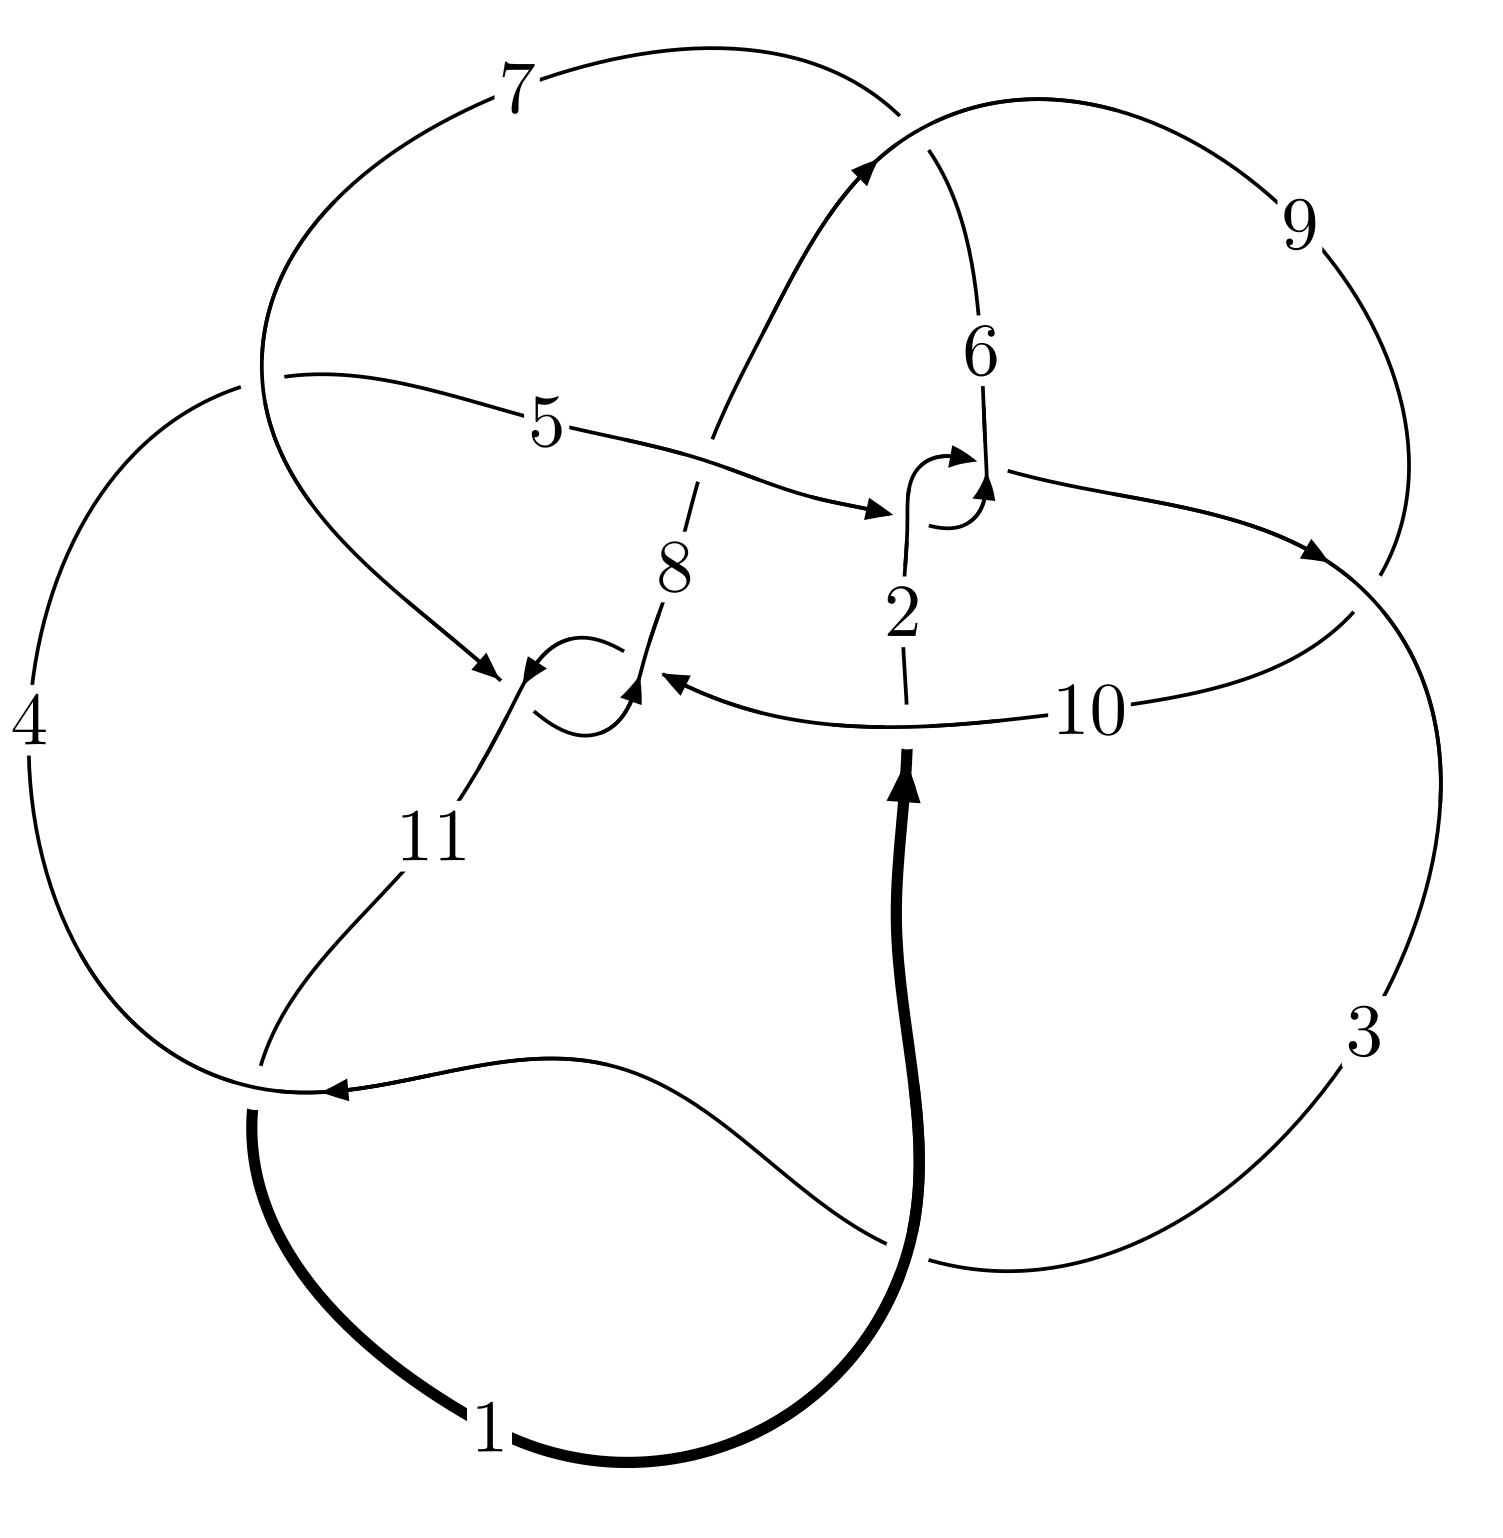
\includegraphics[width=112pt]{../../../GIT/diagram.site/Diagrams/png/552_11a_303.png}\\
\ \ \ A knot diagram\footnotemark}&
\allowdisplaybreaks
\textbf{Linearized knot diagam} \\
\cline{2-2}
 &
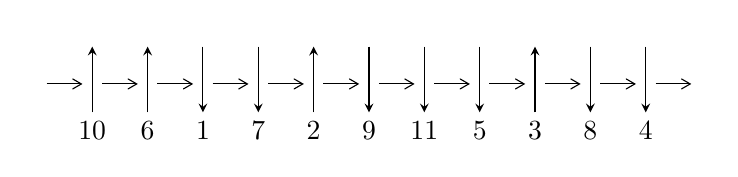
\begin{tikzpicture}[x=20pt, y=17pt]
	% nodes
	\node (C0) at (0, 0) {};
	\node (C1) at (1, 0) {};
	\node (C1U) at (1, +1) {};
	\node (C1D) at (1, -1) {10};

	\node (C2) at (2, 0) {};
	\node (C2U) at (2, +1) {};
	\node (C2D) at (2, -1) {6};

	\node (C3) at (3, 0) {};
	\node (C3U) at (3, +1) {};
	\node (C3D) at (3, -1) {1};

	\node (C4) at (4, 0) {};
	\node (C4U) at (4, +1) {};
	\node (C4D) at (4, -1) {7};

	\node (C5) at (5, 0) {};
	\node (C5U) at (5, +1) {};
	\node (C5D) at (5, -1) {2};

	\node (C6) at (6, 0) {};
	\node (C6U) at (6, +1) {};
	\node (C6D) at (6, -1) {9};

	\node (C7) at (7, 0) {};
	\node (C7U) at (7, +1) {};
	\node (C7D) at (7, -1) {11};

	\node (C8) at (8, 0) {};
	\node (C8U) at (8, +1) {};
	\node (C8D) at (8, -1) {5};

	\node (C9) at (9, 0) {};
	\node (C9U) at (9, +1) {};
	\node (C9D) at (9, -1) {3};

	\node (C10) at (10, 0) {};
	\node (C10U) at (10, +1) {};
	\node (C10D) at (10, -1) {8};

	\node (C11) at (11, 0) {};
	\node (C11U) at (11, +1) {};
	\node (C11D) at (11, -1) {4};
	\node (C12) at (12, 0) {};

	% arrows
	\draw[->,>={angle 60}]
	(C0) edge (C1) (C1) edge (C2) (C2) edge (C3) (C3) edge (C4) (C4) edge (C5) (C5) edge (C6) (C6) edge (C7) (C7) edge (C8) (C8) edge (C9) (C9) edge (C10) (C10) edge (C11) (C11) edge (C12) ;	\draw[->,>=stealth]
	(C1D) edge (C1U) (C2D) edge (C2U) (C3U) edge (C3D) (C4U) edge (C4D) (C5D) edge (C5U) (C6U) edge (C6D) (C7U) edge (C7D) (C8U) edge (C8D) (C9D) edge (C9U) (C10U) edge (C10D) (C11U) edge (C11D) ;
	\end{tikzpicture} \\
\hhline{~~} \\& 
\textbf{Solving Sequence} \\ \cline{2-2} 
 &
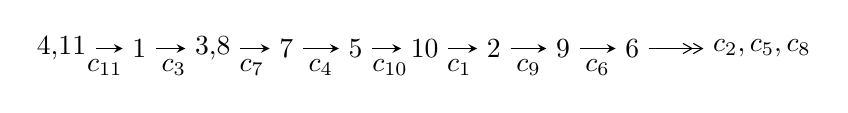
\begin{tikzpicture}[x=25pt, y=7pt]
	% node
	\node (A0) at (-1/8, 0) {4,11};
	\node (A1) at (1, 0) {1};
	\node (A2) at (33/16, 0) {3,8};
	\node (A3) at (25/8, 0) {7};
	\node (A4) at (33/8, 0) {5};
	\node (A5) at (41/8, 0) {10};
	\node (A6) at (49/8, 0) {2};
	\node (A7) at (57/8, 0) {9};
	\node (A8) at (65/8, 0) {6};
	\node (C1) at (1/2, -1) {$c_{11}$};
	\node (C2) at (3/2, -1) {$c_{3}$};
	\node (C3) at (21/8, -1) {$c_{7}$};
	\node (C4) at (29/8, -1) {$c_{4}$};
	\node (C5) at (37/8, -1) {$c_{10}$};
	\node (C6) at (45/8, -1) {$c_{1}$};
	\node (C7) at (53/8, -1) {$c_{9}$};
	\node (C8) at (61/8, -1) {$c_{6}$};
	\node (A9) at (10, 0) {$c_{2},c_{5},c_{8}$};

	% edge
	\draw[->,>=stealth]	
	(A0) edge (A1) (A1) edge (A2) (A2) edge (A3) (A3) edge (A4) (A4) edge (A5) (A5) edge (A6) (A6) edge (A7) (A7) edge (A8) ;
	\draw[->>,>={angle 60}]	
	(A8) edge (A9);
\end{tikzpicture} \\ 

\end{tabular} \\

\footnotetext{
The image of knot diagram is generated by the software ``\textbf{Draw programme}" developed by Andrew Bartholomew(\url{http://www.layer8.co.uk/maths/draw/index.htm\#Running-draw}), where we modified some parts for our purpose(\url{https://github.com/CATsTAILs/LinksPainter}).
}\phantom \\ \newline 
\centering \textbf{Ideals for irreducible components\footnotemark of $X_{\text{par}}$} 
 
\begin{align*}
I^u_{1}&=\langle 
-1.48808\times10^{308} u^{95}+9.86759\times10^{308} u^{94}+\cdots+4.90698\times10^{310} b+6.42779\times10^{310},\\
\phantom{I^u_{1}}&\phantom{= \langle  }-1.38789\times10^{310} u^{95}+6.29806\times10^{310} u^{94}+\cdots+1.55551\times10^{313} a+4.25558\times10^{313},\\
\phantom{I^u_{1}}&\phantom{= \langle  }u^{96}-6 u^{95}+\cdots-1182 u+317\rangle \\
I^u_{2}&=\langle 
-1523509 u^{21}+574654 u^{20}+\cdots+551059 b+558107,\\
\phantom{I^u_{2}}&\phantom{= \langle  }477699 u^{21}+1108403 u^{20}+\cdots+551059 a+2614941,\;u^{22}- u^{21}+\cdots-7 u+1\rangle \\
\\
\end{align*}
\raggedright * 2 irreducible components of $\dim_{\mathbb{C}}=0$, with total 118 representations.\\
\footnotetext{All coefficients of polynomials are rational numbers. But the coefficients are sometimes approximated in decimal forms when there is not enough margin.}
\newpage
\renewcommand{\arraystretch}{1}
\centering \section*{I. $I^u_{1}= \langle -1.49\times10^{308} u^{95}+9.87\times10^{308} u^{94}+\cdots+4.91\times10^{310} b+6.43\times10^{310},\;-1.39\times10^{310} u^{95}+6.30\times10^{310} u^{94}+\cdots+1.56\times10^{313} a+4.26\times10^{313},\;u^{96}-6 u^{95}+\cdots-1182 u+317 \rangle$}
\flushleft \textbf{(i) Arc colorings}\\
\begin{tabular}{m{7pt} m{180pt} m{7pt} m{180pt} }
\flushright $a_{4}=$&$\begin{pmatrix}0\\u\end{pmatrix}$ \\
\flushright $a_{11}=$&$\begin{pmatrix}1\\0\end{pmatrix}$ \\
\flushright $a_{1}=$&$\begin{pmatrix}1\\u^2\end{pmatrix}$ \\
\flushright $a_{3}=$&$\begin{pmatrix}u\\u^3+u\end{pmatrix}$ \\
\flushright $a_{8}=$&$\begin{pmatrix}0.000892242 u^{95}-0.00404887 u^{94}+\cdots-4.66373 u-2.73581\\0.00303257 u^{95}-0.0201093 u^{94}+\cdots+1.71392 u-1.30993\end{pmatrix}$ \\
\flushright $a_{7}=$&$\begin{pmatrix}0.00392481 u^{95}-0.0241582 u^{94}+\cdots-2.94981 u-4.04573\\0.00303257 u^{95}-0.0201093 u^{94}+\cdots+1.71392 u-1.30993\end{pmatrix}$ \\
\flushright $a_{5}=$&$\begin{pmatrix}-0.00516595 u^{95}+0.0454676 u^{94}+\cdots-0.212600 u-0.834715\\0.00767468 u^{95}-0.0509625 u^{94}+\cdots+10.9615 u-2.31606\end{pmatrix}$ \\
\flushright $a_{10}=$&$\begin{pmatrix}0.000339483 u^{95}+0.0120803 u^{94}+\cdots-28.0243 u+3.87884\\0.00696670 u^{95}-0.0482427 u^{94}+\cdots+3.16500 u-1.55323\end{pmatrix}$ \\
\flushright $a_{2}=$&$\begin{pmatrix}0.00900256 u^{95}-0.0295883 u^{94}+\cdots+11.2540 u+2.08466\\-0.00505604 u^{95}+0.0152043 u^{94}+\cdots+15.2711 u-3.72251\end{pmatrix}$ \\
\flushright $a_{9}=$&$\begin{pmatrix}0.00500128 u^{95}-0.0143063 u^{94}+\cdots-26.3933 u+3.66559\\0.00876741 u^{95}-0.0603925 u^{94}+\cdots+5.19063 u-2.26865\end{pmatrix}$ \\
\flushright $a_{6}=$&$\begin{pmatrix}0.00136937 u^{95}-0.0219863 u^{94}+\cdots-12.9762 u-2.37391\\0.00246690 u^{95}-0.0106302 u^{94}+\cdots-4.64789 u+0.104132\end{pmatrix}$\\ \flushright $a_{6}=$&$\begin{pmatrix}0.00136937 u^{95}-0.0219863 u^{94}+\cdots-12.9762 u-2.37391\\0.00246690 u^{95}-0.0106302 u^{94}+\cdots-4.64789 u+0.104132\end{pmatrix}$\\&\end{tabular}
\flushleft \textbf{(ii) Obstruction class $= -1$}\\~\\
\flushleft \textbf{(iii) Cusp Shapes $= -0.0250992 u^{95}+0.186713 u^{94}+\cdots-78.8891 u+8.37508$}\\~\\
\newpage\renewcommand{\arraystretch}{1}
\flushleft \textbf{(iv) u-Polynomials at the component}\newline \\
\begin{tabular}{m{50pt}|m{274pt}}
Crossings & \hspace{64pt}u-Polynomials at each crossing \\
\hline $$\begin{aligned}c_{1}\end{aligned}$$&$\begin{aligned}
&u^{96}+10 u^{95}+\cdots+6633 u+3041
\end{aligned}$\\
\hline $$\begin{aligned}c_{2},c_{5}\end{aligned}$$&$\begin{aligned}
&u^{96}-3 u^{95}+\cdots-94 u+61
\end{aligned}$\\
\hline $$\begin{aligned}c_{3},c_{11}\end{aligned}$$&$\begin{aligned}
&u^{96}-6 u^{95}+\cdots-1182 u+317
\end{aligned}$\\
\hline $$\begin{aligned}c_{4}\end{aligned}$$&$\begin{aligned}
&u^{96}-9 u^{95}+\cdots-16879 u+53041
\end{aligned}$\\
\hline $$\begin{aligned}c_{6}\end{aligned}$$&$\begin{aligned}
&u^{96}-9 u^{95}+\cdots-5684 u+379
\end{aligned}$\\
\hline $$\begin{aligned}c_{7},c_{10}\end{aligned}$$&$\begin{aligned}
&u^{96}+4 u^{95}+\cdots+632 u+589
\end{aligned}$\\
\hline $$\begin{aligned}c_{8}\end{aligned}$$&$\begin{aligned}
&u^{96}+3 u^{95}+\cdots-246 u+157
\end{aligned}$\\
\hline $$\begin{aligned}c_{9}\end{aligned}$$&$\begin{aligned}
&u^{96}-2 u^{95}+\cdots-17198 u+3401
\end{aligned}$\\
\hline
\end{tabular}\\~\\
\newpage\renewcommand{\arraystretch}{1}
\flushleft \textbf{(v) Riley Polynomials at the component}\newline \\
\begin{tabular}{m{50pt}|m{274pt}}
Crossings & \hspace{64pt}Riley Polynomials at each crossing \\
\hline $$\begin{aligned}c_{1}\end{aligned}$$&$\begin{aligned}
&y^{96}-32 y^{95}+\cdots-121986175 y+9247681
\end{aligned}$\\
\hline $$\begin{aligned}c_{2},c_{5}\end{aligned}$$&$\begin{aligned}
&y^{96}-59 y^{95}+\cdots-111072 y+3721
\end{aligned}$\\
\hline $$\begin{aligned}c_{3},c_{11}\end{aligned}$$&$\begin{aligned}
&y^{96}+82 y^{95}+\cdots-4643204 y+100489
\end{aligned}$\\
\hline $$\begin{aligned}c_{4}\end{aligned}$$&$\begin{aligned}
&y^{96}+37 y^{95}+\cdots+73089472791 y+2813347681
\end{aligned}$\\
\hline $$\begin{aligned}c_{6}\end{aligned}$$&$\begin{aligned}
&y^{96}+21 y^{95}+\cdots-49650 y+143641
\end{aligned}$\\
\hline $$\begin{aligned}c_{7},c_{10}\end{aligned}$$&$\begin{aligned}
&y^{96}+64 y^{95}+\cdots+11074296 y+346921
\end{aligned}$\\
\hline $$\begin{aligned}c_{8}\end{aligned}$$&$\begin{aligned}
&y^{96}+3 y^{95}+\cdots+32428 y+24649
\end{aligned}$\\
\hline $$\begin{aligned}c_{9}\end{aligned}$$&$\begin{aligned}
&y^{96}-28 y^{95}+\cdots+255762164 y+11566801
\end{aligned}$\\
\hline
\end{tabular}\\~\\
\newpage\flushleft \textbf{(vi) Complex Volumes and Cusp Shapes}
$$\begin{array}{c|c|c}  
\text{Solutions to }I^u_{1}& \I (\text{vol} + \sqrt{-1}CS) & \text{Cusp shape}\\
 \hline 
\begin{aligned}
u &= -0.525298 + 0.768063 I \\
a &= \phantom{-}0.832846 + 0.127540 I \\
b &= \phantom{-}0.306967 + 0.674805 I\end{aligned}
 & \phantom{-}0.128921 + 1.031740 I & \phantom{-0.000000 } 0 \\ \hline\begin{aligned}
u &= -0.525298 - 0.768063 I \\
a &= \phantom{-}0.832846 - 0.127540 I \\
b &= \phantom{-}0.306967 - 0.674805 I\end{aligned}
 & \phantom{-}0.128921 - 1.031740 I & \phantom{-0.000000 } 0 \\ \hline\begin{aligned}
u &= -0.905763 + 0.203058 I \\
a &= \phantom{-}0.528701 + 0.137906 I \\
b &= -0.368997 - 1.240100 I\end{aligned}
 & \phantom{-}3.35405 - 3.65742 I & \phantom{-0.000000 } 0 \\ \hline\begin{aligned}
u &= -0.905763 - 0.203058 I \\
a &= \phantom{-}0.528701 - 0.137906 I \\
b &= -0.368997 + 1.240100 I\end{aligned}
 & \phantom{-}3.35405 + 3.65742 I & \phantom{-0.000000 } 0 \\ \hline\begin{aligned}
u &= -0.044423 + 1.100350 I \\
a &= \phantom{-}0.670337 - 0.111127 I \\
b &= -1.49263 + 0.17670 I\end{aligned}
 & \phantom{-}0.85043 + 1.34410 I & \phantom{-0.000000 } 0 \\ \hline\begin{aligned}
u &= -0.044423 - 1.100350 I \\
a &= \phantom{-}0.670337 + 0.111127 I \\
b &= -1.49263 - 0.17670 I\end{aligned}
 & \phantom{-}0.85043 - 1.34410 I & \phantom{-0.000000 } 0 \\ \hline\begin{aligned}
u &= \phantom{-}0.156095 + 1.116810 I \\
a &= \phantom{-}0.77783 - 1.99140 I \\
b &= -0.151729 + 1.185900 I\end{aligned}
 & \phantom{-}4.33126 + 2.63781 I & \phantom{-0.000000 } 0 \\ \hline\begin{aligned}
u &= \phantom{-}0.156095 - 1.116810 I \\
a &= \phantom{-}0.77783 + 1.99140 I \\
b &= -0.151729 - 1.185900 I\end{aligned}
 & \phantom{-}4.33126 - 2.63781 I & \phantom{-0.000000 } 0 \\ \hline\begin{aligned}
u &= \phantom{-}0.211266 + 1.131180 I \\
a &= -0.620255 + 0.772149 I \\
b &= -0.728438 - 0.962019 I\end{aligned}
 & \phantom{-}3.97517 - 5.01625 I & \phantom{-0.000000 } 0 \\ \hline\begin{aligned}
u &= \phantom{-}0.211266 - 1.131180 I \\
a &= -0.620255 - 0.772149 I \\
b &= -0.728438 + 0.962019 I\end{aligned}
 & \phantom{-}3.97517 + 5.01625 I & \phantom{-0.000000 } 0\\
 \hline 
 \end{array}$$\newpage$$\begin{array}{c|c|c}  
\text{Solutions to }I^u_{1}& \I (\text{vol} + \sqrt{-1}CS) & \text{Cusp shape}\\
 \hline 
\begin{aligned}
u &= -0.746714 + 0.400699 I \\
a &= -0.051089 - 0.427290 I \\
b &= -0.282677 + 0.880126 I\end{aligned}
 & -0.02117 + 1.72461 I & \phantom{-0.000000 } 0 \\ \hline\begin{aligned}
u &= -0.746714 - 0.400699 I \\
a &= -0.051089 + 0.427290 I \\
b &= -0.282677 - 0.880126 I\end{aligned}
 & -0.02117 - 1.72461 I & \phantom{-0.000000 } 0 \\ \hline\begin{aligned}
u &= -0.431506 + 0.716563 I \\
a &= \phantom{-}0.370722 - 0.216183 I \\
b &= \phantom{-}0.027208 + 0.363722 I\end{aligned}
 & \phantom{-}0.08320 + 1.41662 I & \phantom{-0.000000 } 0 \\ \hline\begin{aligned}
u &= -0.431506 - 0.716563 I \\
a &= \phantom{-}0.370722 + 0.216183 I \\
b &= \phantom{-}0.027208 - 0.363722 I\end{aligned}
 & \phantom{-}0.08320 - 1.41662 I & \phantom{-0.000000 } 0 \\ \hline\begin{aligned}
u &= -0.707791 + 0.931631 I \\
a &= \phantom{-}1.24064 + 0.71963 I \\
b &= \phantom{-}0.251316 - 1.000650 I\end{aligned}
 & \phantom{-}1.15309 + 3.61333 I & \phantom{-0.000000 } 0 \\ \hline\begin{aligned}
u &= -0.707791 - 0.931631 I \\
a &= \phantom{-}1.24064 - 0.71963 I \\
b &= \phantom{-}0.251316 + 1.000650 I\end{aligned}
 & \phantom{-}1.15309 - 3.61333 I & \phantom{-0.000000 } 0 \\ \hline\begin{aligned}
u &= \phantom{-}0.484567 + 1.065950 I \\
a &= -0.382479 - 0.495717 I \\
b &= \phantom{-}0.178676 - 0.553111 I\end{aligned}
 & \phantom{-}4.73513 - 6.35747 I & \phantom{-0.000000 } 0 \\ \hline\begin{aligned}
u &= \phantom{-}0.484567 - 1.065950 I \\
a &= -0.382479 + 0.495717 I \\
b &= \phantom{-}0.178676 + 0.553111 I\end{aligned}
 & \phantom{-}4.73513 + 6.35747 I & \phantom{-0.000000 } 0 \\ \hline\begin{aligned}
u &= -0.247030 + 1.153520 I \\
a &= \phantom{-}0.56682 + 2.45051 I \\
b &= \phantom{-}0.047546 - 1.035870 I\end{aligned}
 & \phantom{-}1.37019 + 2.25364 I & \phantom{-0.000000 } 0 \\ \hline\begin{aligned}
u &= -0.247030 - 1.153520 I \\
a &= \phantom{-}0.56682 - 2.45051 I \\
b &= \phantom{-}0.047546 + 1.035870 I\end{aligned}
 & \phantom{-}1.37019 - 2.25364 I & \phantom{-0.000000 } 0\\
 \hline 
 \end{array}$$\newpage$$\begin{array}{c|c|c}  
\text{Solutions to }I^u_{1}& \I (\text{vol} + \sqrt{-1}CS) & \text{Cusp shape}\\
 \hline 
\begin{aligned}
u &= -0.157639 + 1.183670 I \\
a &= \phantom{-}0.001084 + 0.184832 I \\
b &= -0.832195 + 0.249563 I\end{aligned}
 & \phantom{-}1.92782 + 0.64289 I & \phantom{-0.000000 } 0 \\ \hline\begin{aligned}
u &= -0.157639 - 1.183670 I \\
a &= \phantom{-}0.001084 - 0.184832 I \\
b &= -0.832195 - 0.249563 I\end{aligned}
 & \phantom{-}1.92782 - 0.64289 I & \phantom{-0.000000 } 0 \\ \hline\begin{aligned}
u &= \phantom{-}0.738861 + 0.273522 I \\
a &= \phantom{-}0.657325 + 0.379173 I \\
b &= \phantom{-}0.406156 + 0.380173 I\end{aligned}
 & \phantom{-}2.46146 + 1.79544 I & -1.45895 + 0. I\phantom{ +0.000000I} \\ \hline\begin{aligned}
u &= \phantom{-}0.738861 - 0.273522 I \\
a &= \phantom{-}0.657325 - 0.379173 I \\
b &= \phantom{-}0.406156 - 0.380173 I\end{aligned}
 & \phantom{-}2.46146 - 1.79544 I & -1.45895 + 0. I\phantom{ +0.000000I} \\ \hline\begin{aligned}
u &= \phantom{-}0.179022 + 1.204630 I \\
a &= -0.01303 - 3.15047 I \\
b &= \phantom{-}0.116577 + 1.093260 I\end{aligned}
 & \phantom{-}6.31205 - 7.68822 I & \phantom{-0.000000 } 0 \\ \hline\begin{aligned}
u &= \phantom{-}0.179022 - 1.204630 I \\
a &= -0.01303 + 3.15047 I \\
b &= \phantom{-}0.116577 - 1.093260 I\end{aligned}
 & \phantom{-}6.31205 + 7.68822 I & \phantom{-0.000000 } 0 \\ \hline\begin{aligned}
u &= -0.012622 + 1.218940 I \\
a &= \phantom{-}0.986741 + 0.267737 I \\
b &= -1.43710 - 0.15178 I\end{aligned}
 & \phantom{-}1.37179 - 1.08663 I & \phantom{-0.000000 } 0 \\ \hline\begin{aligned}
u &= -0.012622 - 1.218940 I \\
a &= \phantom{-}0.986741 - 0.267737 I \\
b &= -1.43710 + 0.15178 I\end{aligned}
 & \phantom{-}1.37179 + 1.08663 I & \phantom{-0.000000 } 0 \\ \hline\begin{aligned}
u &= \phantom{-}0.769195 + 0.076746 I \\
a &= \phantom{-}0.501727 + 0.959808 I \\
b &= \phantom{-}0.764067 - 0.172537 I\end{aligned}
 & \phantom{-}1.54996 - 7.35456 I & -3.65767 + 5.46779 I \\ \hline\begin{aligned}
u &= \phantom{-}0.769195 - 0.076746 I \\
a &= \phantom{-}0.501727 - 0.959808 I \\
b &= \phantom{-}0.764067 + 0.172537 I\end{aligned}
 & \phantom{-}1.54996 + 7.35456 I & -3.65767 - 5.46779 I\\
 \hline 
 \end{array}$$\newpage$$\begin{array}{c|c|c}  
\text{Solutions to }I^u_{1}& \I (\text{vol} + \sqrt{-1}CS) & \text{Cusp shape}\\
 \hline 
\begin{aligned}
u &= \phantom{-}0.252248 + 0.723246 I \\
a &= \phantom{-}0.84707 + 1.47573 I \\
b &= -0.788312 - 0.504034 I\end{aligned}
 & \phantom{-}0.30377 - 1.87014 I & \phantom{-0.000000 -}0. + 5.71715 I \\ \hline\begin{aligned}
u &= \phantom{-}0.252248 - 0.723246 I \\
a &= \phantom{-}0.84707 - 1.47573 I \\
b &= -0.788312 + 0.504034 I\end{aligned}
 & \phantom{-}0.30377 + 1.87014 I & \phantom{-0.000000 } 0. - 5.71715 I \\ \hline\begin{aligned}
u &= -0.437620 + 0.614342 I \\
a &= \phantom{-}0.815012 - 0.971132 I \\
b &= -0.719713 + 0.173039 I\end{aligned}
 & -0.041781 + 0.377009 I & -1.80508 + 1.88167 I \\ \hline\begin{aligned}
u &= -0.437620 - 0.614342 I \\
a &= \phantom{-}0.815012 + 0.971132 I \\
b &= -0.719713 - 0.173039 I\end{aligned}
 & -0.041781 - 0.377009 I & -1.80508 - 1.88167 I \\ \hline\begin{aligned}
u &= -0.751709 + 0.055214 I \\
a &= \phantom{-}0.730341 - 0.926417 I \\
b &= \phantom{-}0.517302 + 0.265791 I\end{aligned}
 & -1.73313 + 1.97657 I & -7.36391 - 3.70859 I \\ \hline\begin{aligned}
u &= -0.751709 - 0.055214 I \\
a &= \phantom{-}0.730341 + 0.926417 I \\
b &= \phantom{-}0.517302 - 0.265791 I\end{aligned}
 & -1.73313 - 1.97657 I & -7.36391 + 3.70859 I \\ \hline\begin{aligned}
u &= \phantom{-}0.295341 + 1.238160 I \\
a &= -0.61300 + 1.66487 I \\
b &= -0.57741 - 1.40354 I\end{aligned}
 & \phantom{-}5.09926 - 5.68444 I & \phantom{-0.000000 } 0 \\ \hline\begin{aligned}
u &= \phantom{-}0.295341 - 1.238160 I \\
a &= -0.61300 - 1.66487 I \\
b &= -0.57741 + 1.40354 I\end{aligned}
 & \phantom{-}5.09926 + 5.68444 I & \phantom{-0.000000 } 0 \\ \hline\begin{aligned}
u &= -0.137364 + 1.273180 I \\
a &= -1.19936 - 2.23118 I \\
b &= -0.299431 + 1.353980 I\end{aligned}
 & \phantom{-}10.54150 + 6.15053 I & \phantom{-0.000000 } 0 \\ \hline\begin{aligned}
u &= -0.137364 - 1.273180 I \\
a &= -1.19936 + 2.23118 I \\
b &= -0.299431 - 1.353980 I\end{aligned}
 & \phantom{-}10.54150 - 6.15053 I & \phantom{-0.000000 } 0\\
 \hline 
 \end{array}$$\newpage$$\begin{array}{c|c|c}  
\text{Solutions to }I^u_{1}& \I (\text{vol} + \sqrt{-1}CS) & \text{Cusp shape}\\
 \hline 
\begin{aligned}
u &= \phantom{-}0.639370 + 0.250525 I \\
a &= \phantom{-}0.565116 + 0.474290 I \\
b &= -0.295651 + 1.043140 I\end{aligned}
 & \phantom{-}1.90927 + 2.19671 I & \phantom{-}0.93082 - 1.10813 I \\ \hline\begin{aligned}
u &= \phantom{-}0.639370 - 0.250525 I \\
a &= \phantom{-}0.565116 - 0.474290 I \\
b &= -0.295651 - 1.043140 I\end{aligned}
 & \phantom{-}1.90927 - 2.19671 I & \phantom{-}0.93082 + 1.10813 I \\ \hline\begin{aligned}
u &= \phantom{-}1.268200 + 0.341927 I \\
a &= \phantom{-}0.278974 - 0.564312 I \\
b &= \phantom{-}0.400782 + 1.210640 I\end{aligned}
 & \phantom{-}4.78123 - 11.65630 I & \phantom{-0.000000 } 0 \\ \hline\begin{aligned}
u &= \phantom{-}1.268200 - 0.341927 I \\
a &= \phantom{-}0.278974 + 0.564312 I \\
b &= \phantom{-}0.400782 - 1.210640 I\end{aligned}
 & \phantom{-}4.78123 + 11.65630 I & \phantom{-0.000000 } 0 \\ \hline\begin{aligned}
u &= -0.000655 + 1.317040 I \\
a &= \phantom{-}0.19536 + 1.86854 I \\
b &= \phantom{-}0.48808 - 1.62742 I\end{aligned}
 & \phantom{-}11.30430 - 4.36654 I & \phantom{-0.000000 } 0 \\ \hline\begin{aligned}
u &= -0.000655 - 1.317040 I \\
a &= \phantom{-}0.19536 - 1.86854 I \\
b &= \phantom{-}0.48808 + 1.62742 I\end{aligned}
 & \phantom{-}11.30430 + 4.36654 I & \phantom{-0.000000 } 0 \\ \hline\begin{aligned}
u &= -0.419520 + 1.263720 I \\
a &= -0.46558 - 1.70466 I \\
b &= -0.55012 + 1.56690 I\end{aligned}
 & \phantom{-}6.77870 + 8.49664 I & \phantom{-0.000000 } 0 \\ \hline\begin{aligned}
u &= -0.419520 - 1.263720 I \\
a &= -0.46558 + 1.70466 I \\
b &= -0.55012 - 1.56690 I\end{aligned}
 & \phantom{-}6.77870 - 8.49664 I & \phantom{-0.000000 } 0 \\ \hline\begin{aligned}
u &= \phantom{-}0.544115 + 0.363196 I \\
a &= \phantom{-}0.940669 + 0.668934 I \\
b &= -0.150654 + 0.928303 I\end{aligned}
 & \phantom{-}1.92259 + 2.10317 I & \phantom{-}0.04322 - 3.10406 I \\ \hline\begin{aligned}
u &= \phantom{-}0.544115 - 0.363196 I \\
a &= \phantom{-}0.940669 - 0.668934 I \\
b &= -0.150654 - 0.928303 I\end{aligned}
 & \phantom{-}1.92259 - 2.10317 I & \phantom{-}0.04322 + 3.10406 I\\
 \hline 
 \end{array}$$\newpage$$\begin{array}{c|c|c}  
\text{Solutions to }I^u_{1}& \I (\text{vol} + \sqrt{-1}CS) & \text{Cusp shape}\\
 \hline 
\begin{aligned}
u &= \phantom{-}0.273818 + 1.329490 I \\
a &= \phantom{-}0.051546 - 0.376505 I \\
b &= \phantom{-}0.825894 + 0.224643 I\end{aligned}
 & \phantom{-}7.43575 - 1.63405 I & \phantom{-0.000000 } 0 \\ \hline\begin{aligned}
u &= \phantom{-}0.273818 - 1.329490 I \\
a &= \phantom{-}0.051546 + 0.376505 I \\
b &= \phantom{-}0.825894 - 0.224643 I\end{aligned}
 & \phantom{-}7.43575 + 1.63405 I & \phantom{-0.000000 } 0 \\ \hline\begin{aligned}
u &= \phantom{-}0.059857 + 1.359900 I \\
a &= \phantom{-}0.36449 - 1.63085 I \\
b &= \phantom{-}0.42491 + 1.36679 I\end{aligned}
 & \phantom{-}7.46220 + 0.46211 I & \phantom{-0.000000 } 0 \\ \hline\begin{aligned}
u &= \phantom{-}0.059857 - 1.359900 I \\
a &= \phantom{-}0.36449 + 1.63085 I \\
b &= \phantom{-}0.42491 - 1.36679 I\end{aligned}
 & \phantom{-}7.46220 - 0.46211 I & \phantom{-0.000000 } 0 \\ \hline\begin{aligned}
u &= -0.327054 + 1.326080 I \\
a &= -0.259748 + 0.092424 I \\
b &= \phantom{-}1.100500 + 0.061477 I\end{aligned}
 & \phantom{-}2.65775 + 5.88966 I & \phantom{-0.000000 } 0 \\ \hline\begin{aligned}
u &= -0.327054 - 1.326080 I \\
a &= -0.259748 - 0.092424 I \\
b &= \phantom{-}1.100500 - 0.061477 I\end{aligned}
 & \phantom{-}2.65775 - 5.88966 I & \phantom{-0.000000 } 0 \\ \hline\begin{aligned}
u &= \phantom{-}0.255988 + 1.341720 I \\
a &= -0.161662 - 0.954739 I \\
b &= -0.294743 + 0.280790 I\end{aligned}
 & \phantom{-}5.47557 + 3.41544 I & \phantom{-0.000000 } 0 \\ \hline\begin{aligned}
u &= \phantom{-}0.255988 - 1.341720 I \\
a &= -0.161662 + 0.954739 I \\
b &= -0.294743 - 0.280790 I\end{aligned}
 & \phantom{-}5.47557 - 3.41544 I & \phantom{-0.000000 } 0 \\ \hline\begin{aligned}
u &= \phantom{-}0.326599 + 1.334520 I \\
a &= -0.464224 - 0.182607 I \\
b &= \phantom{-}1.292860 + 0.011178 I\end{aligned}
 & \phantom{-}6.01630 - 11.30650 I & \phantom{-0.000000 } 0 \\ \hline\begin{aligned}
u &= \phantom{-}0.326599 - 1.334520 I \\
a &= -0.464224 + 0.182607 I \\
b &= \phantom{-}1.292860 - 0.011178 I\end{aligned}
 & \phantom{-}6.01630 + 11.30650 I & \phantom{-0.000000 } 0\\
 \hline 
 \end{array}$$\newpage$$\begin{array}{c|c|c}  
\text{Solutions to }I^u_{1}& \I (\text{vol} + \sqrt{-1}CS) & \text{Cusp shape}\\
 \hline 
\begin{aligned}
u &= \phantom{-}1.386100 + 0.123391 I \\
a &= \phantom{-}0.242081 - 0.614254 I \\
b &= \phantom{-}0.094174 + 1.204520 I\end{aligned}
 & \phantom{-}6.84221 + 0.37747 I & \phantom{-0.000000 } 0 \\ \hline\begin{aligned}
u &= \phantom{-}1.386100 - 0.123391 I \\
a &= \phantom{-}0.242081 + 0.614254 I \\
b &= \phantom{-}0.094174 - 1.204520 I\end{aligned}
 & \phantom{-}6.84221 - 0.37747 I & \phantom{-0.000000 } 0 \\ \hline\begin{aligned}
u &= \phantom{-}0.231802 + 1.386730 I \\
a &= -0.33603 + 2.14529 I \\
b &= -0.53021 - 1.50271 I\end{aligned}
 & \phantom{-}7.02857 - 7.75807 I & \phantom{-0.000000 } 0 \\ \hline\begin{aligned}
u &= \phantom{-}0.231802 - 1.386730 I \\
a &= -0.33603 - 2.14529 I \\
b &= -0.53021 + 1.50271 I\end{aligned}
 & \phantom{-}7.02857 + 7.75807 I & \phantom{-0.000000 } 0 \\ \hline\begin{aligned}
u &= \phantom{-}0.546250 + 0.221921 I \\
a &= -0.586107 + 0.400357 I \\
b &= -0.503916 - 1.193030 I\end{aligned}
 & \phantom{-}1.88753 - 4.83574 I & -1.82150 + 10.28229 I \\ \hline\begin{aligned}
u &= \phantom{-}0.546250 - 0.221921 I \\
a &= -0.586107 - 0.400357 I \\
b &= -0.503916 + 1.193030 I\end{aligned}
 & \phantom{-}1.88753 + 4.83574 I & -1.82150 - 10.28229 I \\ \hline\begin{aligned}
u &= -1.351470 + 0.411646 I \\
a &= \phantom{-}0.346166 + 0.613782 I \\
b &= \phantom{-}0.319758 - 1.115460 I\end{aligned}
 & \phantom{-}0.80165 + 5.35661 I & \phantom{-0.000000 } 0 \\ \hline\begin{aligned}
u &= -1.351470 - 0.411646 I \\
a &= \phantom{-}0.346166 - 0.613782 I \\
b &= \phantom{-}0.319758 + 1.115460 I\end{aligned}
 & \phantom{-}0.80165 - 5.35661 I & \phantom{-0.000000 } 0 \\ \hline\begin{aligned}
u &= -0.483414 + 0.287960 I \\
a &= -0.207258 - 0.799988 I \\
b &= -0.829215 + 0.552365 I\end{aligned}
 & -0.78991 + 2.57371 I & -7.44192 - 8.81611 I \\ \hline\begin{aligned}
u &= -0.483414 - 0.287960 I \\
a &= -0.207258 + 0.799988 I \\
b &= -0.829215 - 0.552365 I\end{aligned}
 & -0.78991 - 2.57371 I & -7.44192 + 8.81611 I\\
 \hline 
 \end{array}$$\newpage$$\begin{array}{c|c|c}  
\text{Solutions to }I^u_{1}& \I (\text{vol} + \sqrt{-1}CS) & \text{Cusp shape}\\
 \hline 
\begin{aligned}
u &= \phantom{-}0.17575 + 1.42720 I \\
a &= \phantom{-}0.746124 - 1.151820 I \\
b &= \phantom{-}0.231196 + 0.933301 I\end{aligned}
 & \phantom{-}7.67642 - 0.59175 I & \phantom{-0.000000 } 0 \\ \hline\begin{aligned}
u &= \phantom{-}0.17575 - 1.42720 I \\
a &= \phantom{-}0.746124 + 1.151820 I \\
b &= \phantom{-}0.231196 - 0.933301 I\end{aligned}
 & \phantom{-}7.67642 + 0.59175 I & \phantom{-0.000000 } 0 \\ \hline\begin{aligned}
u &= -0.24656 + 1.42253 I \\
a &= \phantom{-}1.04720 + 1.40871 I \\
b &= \phantom{-}0.027903 - 1.128860 I\end{aligned}
 & \phantom{-}8.87495 + 0.32269 I & \phantom{-0.000000 } 0 \\ \hline\begin{aligned}
u &= -0.24656 - 1.42253 I \\
a &= \phantom{-}1.04720 - 1.40871 I \\
b &= \phantom{-}0.027903 + 1.128860 I\end{aligned}
 & \phantom{-}8.87495 - 0.32269 I & \phantom{-0.000000 } 0 \\ \hline\begin{aligned}
u &= \phantom{-}0.02044 + 1.44372 I \\
a &= \phantom{-}0.076974 + 1.408660 I \\
b &= \phantom{-}0.72037 - 1.26880 I\end{aligned}
 & \phantom{-}9.94869 + 4.20442 I & \phantom{-0.000000 } 0 \\ \hline\begin{aligned}
u &= \phantom{-}0.02044 - 1.44372 I \\
a &= \phantom{-}0.076974 - 1.408660 I \\
b &= \phantom{-}0.72037 + 1.26880 I\end{aligned}
 & \phantom{-}9.94869 - 4.20442 I & \phantom{-0.000000 } 0 \\ \hline\begin{aligned}
u &= \phantom{-}0.415406 + 0.361543 I \\
a &= \phantom{-}2.21587 + 0.61418 I \\
b &= \phantom{-}0.455317 - 0.923063 I\end{aligned}
 & \phantom{-}3.66695 + 5.47402 I & \phantom{-}0.51268 - 6.29867 I \\ \hline\begin{aligned}
u &= \phantom{-}0.415406 - 0.361543 I \\
a &= \phantom{-}2.21587 - 0.61418 I \\
b &= \phantom{-}0.455317 + 0.923063 I\end{aligned}
 & \phantom{-}3.66695 - 5.47402 I & \phantom{-}0.51268 + 6.29867 I \\ \hline\begin{aligned}
u &= -0.28768 + 1.44338 I \\
a &= -0.21246 - 1.79678 I \\
b &= -0.51281 + 1.38469 I\end{aligned}
 & \phantom{-}5.80229 + 5.49787 I & \phantom{-0.000000 } 0 \\ \hline\begin{aligned}
u &= -0.28768 - 1.44338 I \\
a &= -0.21246 + 1.79678 I \\
b &= -0.51281 - 1.38469 I\end{aligned}
 & \phantom{-}5.80229 - 5.49787 I & \phantom{-0.000000 } 0\\
 \hline 
 \end{array}$$\newpage$$\begin{array}{c|c|c}  
\text{Solutions to }I^u_{1}& \I (\text{vol} + \sqrt{-1}CS) & \text{Cusp shape}\\
 \hline 
\begin{aligned}
u &= \phantom{-}0.52488 + 1.47047 I \\
a &= \phantom{-}0.75954 - 1.52436 I \\
b &= \phantom{-}0.402301 + 1.326180 I\end{aligned}
 & \phantom{-}12.08550 - 6.02777 I & \phantom{-0.000000 } 0 \\ \hline\begin{aligned}
u &= \phantom{-}0.52488 - 1.47047 I \\
a &= \phantom{-}0.75954 + 1.52436 I \\
b &= \phantom{-}0.402301 - 1.326180 I\end{aligned}
 & \phantom{-}12.08550 + 6.02777 I & \phantom{-0.000000 } 0 \\ \hline\begin{aligned}
u &= \phantom{-}0.49192 + 1.51520 I \\
a &= \phantom{-}0.52792 - 1.65271 I \\
b &= \phantom{-}0.57582 + 1.42748 I\end{aligned}
 & \phantom{-}10.6115 - 17.7790 I & \phantom{-0.000000 } 0 \\ \hline\begin{aligned}
u &= \phantom{-}0.49192 - 1.51520 I \\
a &= \phantom{-}0.52792 + 1.65271 I \\
b &= \phantom{-}0.57582 - 1.42748 I\end{aligned}
 & \phantom{-}10.6115 + 17.7790 I & \phantom{-0.000000 } 0 \\ \hline\begin{aligned}
u &= -0.50869 + 1.52093 I \\
a &= \phantom{-}0.56522 + 1.55059 I \\
b &= \phantom{-}0.54425 - 1.34959 I\end{aligned}
 & \phantom{-}6.73423 + 11.71500 I & \phantom{-0.000000 } 0 \\ \hline\begin{aligned}
u &= -0.50869 - 1.52093 I \\
a &= \phantom{-}0.56522 - 1.55059 I \\
b &= \phantom{-}0.54425 + 1.34959 I\end{aligned}
 & \phantom{-}6.73423 - 11.71500 I & \phantom{-0.000000 } 0 \\ \hline\begin{aligned}
u &= \phantom{-}0.57035 + 1.51967 I \\
a &= -0.47162 + 1.46962 I \\
b &= -0.19365 - 1.44897 I\end{aligned}
 & \phantom{-}11.70320 - 7.44211 I & \phantom{-0.000000 } 0 \\ \hline\begin{aligned}
u &= \phantom{-}0.57035 - 1.51967 I \\
a &= -0.47162 - 1.46962 I \\
b &= -0.19365 + 1.44897 I\end{aligned}
 & \phantom{-}11.70320 + 7.44211 I & \phantom{-0.000000 } 0 \\ \hline\begin{aligned}
u &= \phantom{-}0.278450 + 0.071670 I \\
a &= -1.52137 + 0.64328 I \\
b &= -0.755950 - 0.092790 I\end{aligned}
 & -1.43035 - 0.01918 I & -9.48323 - 0.92177 I \\ \hline\begin{aligned}
u &= \phantom{-}0.278450 - 0.071670 I \\
a &= -1.52137 - 0.64328 I \\
b &= -0.755950 + 0.092790 I\end{aligned}
 & -1.43035 + 0.01918 I & -9.48323 + 0.92177 I\\
 \hline 
 \end{array}$$\newpage$$\begin{array}{c|c|c}  
\text{Solutions to }I^u_{1}& \I (\text{vol} + \sqrt{-1}CS) & \text{Cusp shape}\\
 \hline 
\begin{aligned}
u &= -0.183899 + 0.086824 I \\
a &= -0.75076 - 4.63928 I \\
b &= \phantom{-}0.022216 - 1.324870 I\end{aligned}
 & \phantom{-}6.79043 - 4.75561 I & \phantom{-}3.73976 + 5.73901 I \\ \hline\begin{aligned}
u &= -0.183899 - 0.086824 I \\
a &= -0.75076 + 4.63928 I \\
b &= \phantom{-}0.022216 + 1.324870 I\end{aligned}
 & \phantom{-}6.79043 + 4.75561 I & \phantom{-}3.73976 - 5.73901 I \\ \hline\begin{aligned}
u &= -0.28859 + 1.82446 I \\
a &= -0.139870 - 1.338690 I \\
b &= -0.262443 + 1.128520 I\end{aligned}
 & \phantom{-}5.90628 + 4.32377 I & \phantom{-0.000000 } 0 \\ \hline\begin{aligned}
u &= -0.28859 - 1.82446 I \\
a &= -0.139870 + 1.338690 I \\
b &= -0.262443 - 1.128520 I\end{aligned}
 & \phantom{-}5.90628 - 4.32377 I & \phantom{-0.000000 } 0 \\ \hline\begin{aligned}
u &= \phantom{-}1.10712 + 1.84505 I \\
a &= -0.305270 + 1.010260 I \\
b &= \phantom{-}0.015849 - 1.136460 I\end{aligned}
 & \phantom{-}7.84962 + 3.05507 I & \phantom{-0.000000 } 0 \\ \hline\begin{aligned}
u &= \phantom{-}1.10712 - 1.84505 I \\
a &= -0.305270 - 1.010260 I \\
b &= \phantom{-}0.015849 + 1.136460 I\end{aligned}
 & \phantom{-}7.84962 - 3.05507 I & \phantom{-0.000000 } 0\\
 \hline 
 \end{array}$$\newpage\newpage\renewcommand{\arraystretch}{1}
\centering \section*{II. $I^u_{2}= \langle -1.52\times10^{6} u^{21}+5.75\times10^{5} u^{20}+\cdots+5.51\times10^{5} b+5.58\times10^{5},\;4.78\times10^{5} u^{21}+1.11\times10^{6} u^{20}+\cdots+5.51\times10^{5} a+2.61\times10^{6},\;u^{22}- u^{21}+\cdots-7 u+1 \rangle$}
\flushleft \textbf{(i) Arc colorings}\\
\begin{tabular}{m{7pt} m{180pt} m{7pt} m{180pt} }
\flushright $a_{4}=$&$\begin{pmatrix}0\\u\end{pmatrix}$ \\
\flushright $a_{11}=$&$\begin{pmatrix}1\\0\end{pmatrix}$ \\
\flushright $a_{1}=$&$\begin{pmatrix}1\\u^2\end{pmatrix}$ \\
\flushright $a_{3}=$&$\begin{pmatrix}u\\u^3+u\end{pmatrix}$ \\
\flushright $a_{8}=$&$\begin{pmatrix}-0.866875 u^{21}-2.01141 u^{20}+\cdots+31.0423 u-4.74530\\2.76469 u^{21}-1.04282 u^{20}+\cdots+7.59317 u-1.01279\end{pmatrix}$ \\
\flushright $a_{7}=$&$\begin{pmatrix}1.89782 u^{21}-3.05422 u^{20}+\cdots+38.6355 u-5.75809\\2.76469 u^{21}-1.04282 u^{20}+\cdots+7.59317 u-1.01279\end{pmatrix}$ \\
\flushright $a_{5}=$&$\begin{pmatrix}-1.36561 u^{21}-3.35513 u^{20}+\cdots+29.1644 u-4.25179\\0.738879 u^{21}-0.454115 u^{20}+\cdots+2.62218 u+0.546192\end{pmatrix}$ \\
\flushright $a_{10}=$&$\begin{pmatrix}-2.20771 u^{21}+1.20618 u^{20}+\cdots-11.3065 u+3.27600\\1.66152 u^{21}+0.0788899 u^{20}+\cdots-10.4549 u+3.16953\end{pmatrix}$ \\
\flushright $a_{2}=$&$\begin{pmatrix}-4.79637 u^{21}+2.41999 u^{20}+\cdots-12.0899 u-0.812203\\-1.28214 u^{21}-0.327382 u^{20}+\cdots-6.66408 u+1.42918\end{pmatrix}$ \\
\flushright $a_{9}=$&$\begin{pmatrix}-3.31089 u^{21}+2.32789 u^{20}+\cdots-29.3545 u+6.45832\\1.02103 u^{21}+1.05286 u^{20}+\cdots-27.2700 u+6.33331\end{pmatrix}$ \\
\flushright $a_{6}=$&$\begin{pmatrix}0.897819 u^{21}-2.05422 u^{20}+\cdots+11.6355 u+0.241909\\0.817375 u^{21}-0.0709815 u^{20}+\cdots+8.84560 u-1.61137\end{pmatrix}$\\ \flushright $a_{6}=$&$\begin{pmatrix}0.897819 u^{21}-2.05422 u^{20}+\cdots+11.6355 u+0.241909\\0.817375 u^{21}-0.0709815 u^{20}+\cdots+8.84560 u-1.61137\end{pmatrix}$\\&\end{tabular}
\flushleft \textbf{(ii) Obstruction class $= 1$}\\~\\
\flushleft \textbf{(iii) Cusp Shapes $= \frac{569868}{551059} u^{21}-\frac{982528}{551059} u^{20}+\cdots-\frac{31980159}{551059} u+\frac{3277033}{551059}$}\\~\\
\newpage\renewcommand{\arraystretch}{1}
\flushleft \textbf{(iv) u-Polynomials at the component}\newline \\
\begin{tabular}{m{50pt}|m{274pt}}
Crossings & \hspace{64pt}u-Polynomials at each crossing \\
\hline $$\begin{aligned}c_{1}\end{aligned}$$&$\begin{aligned}
&u^{22}-3 u^{21}+\cdots-4 u+1
\end{aligned}$\\
\hline $$\begin{aligned}c_{2}\end{aligned}$$&$\begin{aligned}
&u^{22}+2 u^{21}+\cdots+7 u+3
\end{aligned}$\\
\hline $$\begin{aligned}c_{3}\end{aligned}$$&$\begin{aligned}
&u^{22}+u^{21}+\cdots+7 u+1
\end{aligned}$\\
\hline $$\begin{aligned}c_{4}\end{aligned}$$&$\begin{aligned}
&u^{22}+4 u^{19}+\cdots-6 u+1
\end{aligned}$\\
\hline $$\begin{aligned}c_{5}\end{aligned}$$&$\begin{aligned}
&u^{22}-2 u^{21}+\cdots-7 u+3
\end{aligned}$\\
\hline $$\begin{aligned}c_{6}\end{aligned}$$&$\begin{aligned}
&u^{22}-2 u^{21}+\cdots- u+1
\end{aligned}$\\
\hline $$\begin{aligned}c_{7}\end{aligned}$$&$\begin{aligned}
&u^{22}-9 u^{21}+\cdots-23 u+3
\end{aligned}$\\
\hline $$\begin{aligned}c_{8}\end{aligned}$$&$\begin{aligned}
&u^{22}-2 u^{21}+\cdots+3 u+1
\end{aligned}$\\
\hline $$\begin{aligned}c_{9}\end{aligned}$$&$\begin{aligned}
&u^{22}- u^{21}+\cdots- u+1
\end{aligned}$\\
\hline $$\begin{aligned}c_{10}\end{aligned}$$&$\begin{aligned}
&u^{22}+9 u^{21}+\cdots+23 u+3
\end{aligned}$\\
\hline $$\begin{aligned}c_{11}\end{aligned}$$&$\begin{aligned}
&u^{22}- u^{21}+\cdots-7 u+1
\end{aligned}$\\
\hline
\end{tabular}\\~\\
\newpage\renewcommand{\arraystretch}{1}
\flushleft \textbf{(v) Riley Polynomials at the component}\newline \\
\begin{tabular}{m{50pt}|m{274pt}}
Crossings & \hspace{64pt}Riley Polynomials at each crossing \\
\hline $$\begin{aligned}c_{1}\end{aligned}$$&$\begin{aligned}
&y^{22}-13 y^{21}+\cdots+4 y+1
\end{aligned}$\\
\hline $$\begin{aligned}c_{2},c_{5}\end{aligned}$$&$\begin{aligned}
&y^{22}-12 y^{21}+\cdots-85 y+9
\end{aligned}$\\
\hline $$\begin{aligned}c_{3},c_{11}\end{aligned}$$&$\begin{aligned}
&y^{22}+21 y^{21}+\cdots+7 y+1
\end{aligned}$\\
\hline $$\begin{aligned}c_{4}\end{aligned}$$&$\begin{aligned}
&y^{22}+6 y^{20}+\cdots-2 y+1
\end{aligned}$\\
\hline $$\begin{aligned}c_{6}\end{aligned}$$&$\begin{aligned}
&y^{22}-8 y^{21}+\cdots-11 y+1
\end{aligned}$\\
\hline $$\begin{aligned}c_{7},c_{10}\end{aligned}$$&$\begin{aligned}
&y^{22}+11 y^{21}+\cdots+59 y+9
\end{aligned}$\\
\hline $$\begin{aligned}c_{8}\end{aligned}$$&$\begin{aligned}
&y^{22}-6 y^{21}+\cdots-5 y+1
\end{aligned}$\\
\hline $$\begin{aligned}c_{9}\end{aligned}$$&$\begin{aligned}
&y^{22}+3 y^{21}+\cdots-9 y+1
\end{aligned}$\\
\hline
\end{tabular}\\~\\
\newpage\flushleft \textbf{(vi) Complex Volumes and Cusp Shapes}
$$\begin{array}{c|c|c}  
\text{Solutions to }I^u_{2}& \I (\text{vol} + \sqrt{-1}CS) & \text{Cusp shape}\\
 \hline 
\begin{aligned}
u &= -0.325722 + 0.924836 I \\
a &= -0.314978 - 1.013920 I \\
b &= \phantom{-}0.231197 - 0.644969 I\end{aligned}
 & \phantom{-}4.63455 + 7.30143 I & \phantom{-}0.41543 - 9.60759 I \\ \hline\begin{aligned}
u &= -0.325722 - 0.924836 I \\
a &= -0.314978 + 1.013920 I \\
b &= \phantom{-}0.231197 + 0.644969 I\end{aligned}
 & \phantom{-}4.63455 - 7.30143 I & \phantom{-}0.41543 + 9.60759 I \\ \hline\begin{aligned}
u &= \phantom{-}0.751922 + 0.704622 I \\
a &= -1.144800 + 0.379579 I \\
b &= -0.295783 - 1.049270 I\end{aligned}
 & \phantom{-}1.32512 - 4.05365 I & \phantom{-}2.20928 + 9.99112 I \\ \hline\begin{aligned}
u &= \phantom{-}0.751922 - 0.704622 I \\
a &= -1.144800 - 0.379579 I \\
b &= -0.295783 + 1.049270 I\end{aligned}
 & \phantom{-}1.32512 + 4.05365 I & \phantom{-}2.20928 - 9.99112 I \\ \hline\begin{aligned}
u &= \phantom{-}0.329954 + 0.830831 I \\
a &= \phantom{-}0.114259 + 0.430464 I \\
b &= -0.630595 + 0.054388 I\end{aligned}
 & -0.77711 - 1.51881 I & -7.69357 + 3.97599 I \\ \hline\begin{aligned}
u &= \phantom{-}0.329954 - 0.830831 I \\
a &= \phantom{-}0.114259 - 0.430464 I \\
b &= -0.630595 - 0.054388 I\end{aligned}
 & -0.77711 + 1.51881 I & -7.69357 - 3.97599 I \\ \hline\begin{aligned}
u &= \phantom{-}0.028518 + 1.221960 I \\
a &= \phantom{-}0.900081 - 0.223546 I \\
b &= -1.53702 + 0.22214 I\end{aligned}
 & \phantom{-}1.83081 + 0.86562 I & \phantom{-}9.02771 + 1.15882 I \\ \hline\begin{aligned}
u &= \phantom{-}0.028518 - 1.221960 I \\
a &= \phantom{-}0.900081 + 0.223546 I \\
b &= -1.53702 - 0.22214 I\end{aligned}
 & \phantom{-}1.83081 - 0.86562 I & \phantom{-}9.02771 - 1.15882 I \\ \hline\begin{aligned}
u &= \phantom{-}0.361208 + 0.645420 I \\
a &= -1.55687 + 0.56837 I \\
b &= -0.221210 + 0.639754 I\end{aligned}
 & -0.16641 - 1.41041 I & -7.38985 + 6.70652 I \\ \hline\begin{aligned}
u &= \phantom{-}0.361208 - 0.645420 I \\
a &= -1.55687 - 0.56837 I \\
b &= -0.221210 - 0.639754 I\end{aligned}
 & -0.16641 + 1.41041 I & -7.38985 - 6.70652 I\\
 \hline 
 \end{array}$$\newpage$$\begin{array}{c|c|c}  
\text{Solutions to }I^u_{2}& \I (\text{vol} + \sqrt{-1}CS) & \text{Cusp shape}\\
 \hline 
\begin{aligned}
u &= -0.297298 + 1.256540 I \\
a &= -0.74638 - 2.15779 I \\
b &= -0.25149 + 1.46113 I\end{aligned}
 & \phantom{-}8.91096 + 6.90073 I & \phantom{-}4.68084 - 6.27490 I \\ \hline\begin{aligned}
u &= -0.297298 - 1.256540 I \\
a &= -0.74638 + 2.15779 I \\
b &= -0.25149 - 1.46113 I\end{aligned}
 & \phantom{-}8.91096 - 6.90073 I & \phantom{-}4.68084 + 6.27490 I \\ \hline\begin{aligned}
u &= \phantom{-}0.259751 + 1.370260 I \\
a &= -0.30722 + 1.85435 I \\
b &= -0.59274 - 1.48164 I\end{aligned}
 & \phantom{-}6.44412 - 6.53950 I & \phantom{-}3.13648 + 5.18044 I \\ \hline\begin{aligned}
u &= \phantom{-}0.259751 - 1.370260 I \\
a &= -0.30722 - 1.85435 I \\
b &= -0.59274 + 1.48164 I\end{aligned}
 & \phantom{-}6.44412 + 6.53950 I & \phantom{-}3.13648 - 5.18044 I \\ \hline\begin{aligned}
u &= \phantom{-}0.115142 + 0.583729 I \\
a &= \phantom{-}1.17843 + 0.84891 I \\
b &= -0.954267 - 0.339130 I\end{aligned}
 & -0.49687 - 1.33027 I & -8.40153 + 3.08936 I \\ \hline\begin{aligned}
u &= \phantom{-}0.115142 - 0.583729 I \\
a &= \phantom{-}1.17843 - 0.84891 I \\
b &= -0.954267 + 0.339130 I\end{aligned}
 & -0.49687 + 1.33027 I & -8.40153 - 3.08936 I \\ \hline\begin{aligned}
u &= -0.83136 + 1.32090 I \\
a &= \phantom{-}0.367088 + 0.859047 I \\
b &= \phantom{-}0.071362 - 1.159550 I\end{aligned}
 & \phantom{-}7.43077 - 2.45676 I & \phantom{-}4.44661 - 0.13361 I \\ \hline\begin{aligned}
u &= -0.83136 - 1.32090 I \\
a &= \phantom{-}0.367088 - 0.859047 I \\
b &= \phantom{-}0.071362 + 1.159550 I\end{aligned}
 & \phantom{-}7.43077 + 2.45676 I & \phantom{-}4.44661 + 0.13361 I \\ \hline\begin{aligned}
u &= \phantom{-}0.384833 + 0.166221 I \\
a &= \phantom{-}1.47985 + 0.70605 I \\
b &= -0.489921 + 1.129880 I\end{aligned}
 & \phantom{-}2.05850 + 3.60374 I & -1.99861 - 4.85808 I \\ \hline\begin{aligned}
u &= \phantom{-}0.384833 - 0.166221 I \\
a &= \phantom{-}1.47985 - 0.70605 I \\
b &= -0.489921 - 1.129880 I\end{aligned}
 & \phantom{-}2.05850 - 3.60374 I & -1.99861 + 4.85808 I\\
 \hline 
 \end{array}$$\newpage$$\begin{array}{c|c|c}  
\text{Solutions to }I^u_{2}& \I (\text{vol} + \sqrt{-1}CS) & \text{Cusp shape}\\
 \hline 
\begin{aligned}
u &= -0.27695 + 1.72488 I \\
a &= \phantom{-}0.03055 - 1.49682 I \\
b &= \phantom{-}0.170469 + 1.002220 I\end{aligned}
 & \phantom{-}6.63906 - 3.73323 I & \phantom{-}7.06721 + 4.27420 I \\ \hline\begin{aligned}
u &= -0.27695 - 1.72488 I \\
a &= \phantom{-}0.03055 + 1.49682 I \\
b &= \phantom{-}0.170469 - 1.002220 I\end{aligned}
 & \phantom{-}6.63906 + 3.73323 I & \phantom{-}7.06721 - 4.27420 I\\
 \hline 
 \end{array}$$\newpage
\newpage\renewcommand{\arraystretch}{1}
\centering \section*{ III. u-Polynomials}
\begin{tabular}{m{50pt}|m{274pt}}
Crossings & \hspace{64pt}u-Polynomials at each crossing \\
\hline $$\begin{aligned}c_{1}\end{aligned}$$&$\begin{aligned}
&(u^{22}-3 u^{21}+\cdots-4 u+1)(u^{96}+10 u^{95}+\cdots+6633 u+3041)
\end{aligned}$\\
\hline $$\begin{aligned}c_{2}\end{aligned}$$&$\begin{aligned}
&(u^{22}+2 u^{21}+\cdots+7 u+3)(u^{96}-3 u^{95}+\cdots-94 u+61)
\end{aligned}$\\
\hline $$\begin{aligned}c_{3}\end{aligned}$$&$\begin{aligned}
&(u^{22}+u^{21}+\cdots+7 u+1)(u^{96}-6 u^{95}+\cdots-1182 u+317)
\end{aligned}$\\
\hline $$\begin{aligned}c_{4}\end{aligned}$$&$\begin{aligned}
&(u^{22}+4 u^{19}+\cdots-6 u+1)(u^{96}-9 u^{95}+\cdots-16879 u+53041)
\end{aligned}$\\
\hline $$\begin{aligned}c_{5}\end{aligned}$$&$\begin{aligned}
&(u^{22}-2 u^{21}+\cdots-7 u+3)(u^{96}-3 u^{95}+\cdots-94 u+61)
\end{aligned}$\\
\hline $$\begin{aligned}c_{6}\end{aligned}$$&$\begin{aligned}
&(u^{22}-2 u^{21}+\cdots- u+1)(u^{96}-9 u^{95}+\cdots-5684 u+379)
\end{aligned}$\\
\hline $$\begin{aligned}c_{7}\end{aligned}$$&$\begin{aligned}
&(u^{22}-9 u^{21}+\cdots-23 u+3)(u^{96}+4 u^{95}+\cdots+632 u+589)
\end{aligned}$\\
\hline $$\begin{aligned}c_{8}\end{aligned}$$&$\begin{aligned}
&(u^{22}-2 u^{21}+\cdots+3 u+1)(u^{96}+3 u^{95}+\cdots-246 u+157)
\end{aligned}$\\
\hline $$\begin{aligned}c_{9}\end{aligned}$$&$\begin{aligned}
&(u^{22}- u^{21}+\cdots- u+1)(u^{96}-2 u^{95}+\cdots-17198 u+3401)
\end{aligned}$\\
\hline $$\begin{aligned}c_{10}\end{aligned}$$&$\begin{aligned}
&(u^{22}+9 u^{21}+\cdots+23 u+3)(u^{96}+4 u^{95}+\cdots+632 u+589)
\end{aligned}$\\
\hline $$\begin{aligned}c_{11}\end{aligned}$$&$\begin{aligned}
&(u^{22}- u^{21}+\cdots-7 u+1)(u^{96}-6 u^{95}+\cdots-1182 u+317)
\end{aligned}$\\
\hline
\end{tabular}\newpage\renewcommand{\arraystretch}{1}
\centering \section*{ IV. Riley Polynomials}
\begin{tabular}{m{50pt}|m{274pt}}
Crossings & \hspace{64pt}Riley Polynomials at each crossing \\
\hline $$\begin{aligned}c_{1}\end{aligned}$$&$\begin{aligned}
&(y^{22}-13 y^{21}+\cdots+4 y+1)\\
&\cdot(y^{96}-32 y^{95}+\cdots-121986175 y+9247681)
\end{aligned}$\\
\hline $$\begin{aligned}c_{2},c_{5}\end{aligned}$$&$\begin{aligned}
&(y^{22}-12 y^{21}+\cdots-85 y+9)(y^{96}-59 y^{95}+\cdots-111072 y+3721)
\end{aligned}$\\
\hline $$\begin{aligned}c_{3},c_{11}\end{aligned}$$&$\begin{aligned}
&(y^{22}+21 y^{21}+\cdots+7 y+1)(y^{96}+82 y^{95}+\cdots-4643204 y+100489)
\end{aligned}$\\
\hline $$\begin{aligned}c_{4}\end{aligned}$$&$\begin{aligned}
&(y^{22}+6 y^{20}+\cdots-2 y+1)\\
&\cdot(y^{96}+37 y^{95}+\cdots+73089472791 y+2813347681)
\end{aligned}$\\
\hline $$\begin{aligned}c_{6}\end{aligned}$$&$\begin{aligned}
&(y^{22}-8 y^{21}+\cdots-11 y+1)(y^{96}+21 y^{95}+\cdots-49650 y+143641)
\end{aligned}$\\
\hline $$\begin{aligned}c_{7},c_{10}\end{aligned}$$&$\begin{aligned}
&(y^{22}+11 y^{21}+\cdots+59 y+9)\\
&\cdot(y^{96}+64 y^{95}+\cdots+11074296 y+346921)
\end{aligned}$\\
\hline $$\begin{aligned}c_{8}\end{aligned}$$&$\begin{aligned}
&(y^{22}-6 y^{21}+\cdots-5 y+1)(y^{96}+3 y^{95}+\cdots+32428 y+24649)
\end{aligned}$\\
\hline $$\begin{aligned}c_{9}\end{aligned}$$&$\begin{aligned}
&(y^{22}+3 y^{21}+\cdots-9 y+1)\\
&\cdot(y^{96}-28 y^{95}+\cdots+255762164 y+11566801)
\end{aligned}$\\
\hline
\end{tabular}
\vskip 2pc
\end{document}